The Methods section provides an overview of the methodologies employed in the \texttt{PPG-BP} project.
It encompasses various subdirectories such as MIMIC and PyTorch tutorials, with the primary code located within the \texttt{model} Python Package.
Within the \texttt{model}, there exist several sub-packages containing relevant data for subsequent project components,
while the core code is distributed across five \texttt{.py} classes: \texttt{init\_scripts.py} (Initialization / Data Fetching), \texttt{sp\_scripts.py} (Signal Processing),
\texttt{ml\_scripts.py} (Machine Learning), \texttt{visual.py} (Visualization), and \texttt{main.py}, which integrates all the aforementioned components.
The whole repository can be found on the author's \textit{GitHub} page~\cite{jasinskasHtjasPPGBP2024}.

\subsection{Data Fetching}
\label{subsec:data-fetching}

The initial phase in virtually all Data Science endeavors involves Data Preparation.
This section will examine the \texttt{init\_scripts.py} class.
For this project, data was sourced from the MIMIC-III and MIMIC-IV DBs, each serving distinct purposes.
Data from the MIMIC-IV DB was employed as the validation dataset (detailed further in the ML methods section~\ref{subsec:ml_methods}), since it is regarded as the most modern and most reliable MIMIC DB currently available.
In contrast, data from the MIMIC-III database was utilized for training and testing ML models due to its significantly larger size.
Nevertheless, the data retrieval process employed similar methods for both the older and newer waveform datasets.

% Libraries
\vspace{0.2cm}
\textit{Tools and Approaches}
\vspace{0.2cm}

Researchers at the MIT Laboratory for Computational Physiology have developed a native Python library named the waveform-database (WFDB) package, facilitating the convenient handling of MIMIC datasets.
This library comprises tools for reading, writing, and processing WFDB signals and annotations~\cite{MITLCPWfdbpython2024}.
Efficient and consistent data retrieval was achieved through a combination of pre-existing WFDB library functions and custom-written methods.

First of all, a list of all records from the selected DB were fetched utilizing the

\vspace{0.1cm}
{\centering \texttt{wfdb.get\_record\_list(db\_name)}\par}
\vspace{0.1cm}

\noindent method.
Then an iterative process followed, going through all the subjects from the loaded records list.
When assessing a single subject, the same method, but with more specific parameters

\vspace{0.1cm}
{\centering \texttt{wfdb.get\_record\_list((f'{db\_name}/{subject}')}\par}
\vspace{0.1cm}

\noindent was called, in this instance to load all studies from a single subject.
Another loop was formed to iterate through each study within the subject.
These studies consist of records, each representing a single ICU \enquote{session}, during which the patient was connected to at least one monitoring device, therefore they highly differ in time length.
Given the diversity of monitoring devices, these records encompass various signals, including ECG, ABP, and Pleth (equivalent to PPG).
To verify if the record includes all the required signals (ABP and Pleth for this study), the method

\vspace{0.1cm}
{\centering \texttt{record\_data = wfdb.rdheader(subject.name, record\_dir, rd\_segments=True)}\par}
\vspace{0.1cm}

\noindent was invoked, providing the header data of a single record, which is then used to fetch all present signals

\vspace{0.1cm}
{\centering \texttt{signal\_names = record\_data.sig\_name}.\par}
\vspace{0.1cm}

\noindent If the record lacks either the \textit{ABP} or \textit{Pleth} signals, it is excluded from further processing.
However, even a single record comprises multiple segments, varying in duration and the signals they capture.
If a record lacks either the ABP or Pleth signals, it is excluded from further processing.
Each record comprises multiple segments, varying in duration and the signals they capture.
In addition to signal requirements, segments must also have a minimum length of 10 minutes to be considered usable.
This criterion aims to ensure data reliability and variability, as longer segments offer more data points to represent physiological states accurately, reducing the impact of short-term fluctuations and noise.
The segment duration length is determined by the following function:

\vspace{0.1cm}
\qquad\qquad\qquad \texttt{segment\_metadata = wfdb.rdheader(segment, record\_dir)}

\qquad\qquad\qquad \texttt{tot\_seg\_length = segment\_metadata.sig\_len}

\qquad\qquad\qquad \texttt{sampling\_rate = segment\_metadata.fs}

\qquad\qquad\qquad \texttt{seg\_duration = tot\_seg\_length / fs}
\vspace{0.1cm}

\noindent Precisely these segments represent the smallest data samples utilized in this study, containing continuous numeric values sampled at a specific frequency rate.
The data abstraction levels in MIMIC DBs can be depicted by the chart, showing a descending order from left to right:

\vspace{0.1cm}
{\centering \textit{Subject} $\rightarrow$ Study $\rightarrow$ Record $\rightarrow$ Segment\par}
\vspace{0.1cm}

An iterative process is likewise applied to every segment of a record, by fetching all values from a single segment:

\vspace{0.1cm}
{\centering \texttt{segment\_data = wfdb.rdrecord(segment, record\_dir)}.\par}
\vspace{0.1cm}

\noindent These segments should also be devoid of any \enquote{faulty} values, identified as NumPy values \texttt{NaN} and \texttt{inf}.
For ABP segments values outside the range of 30 to 250 (accounting for extreme and likely erroneous measurements) are omitted, and for Pleth values must strictly fall between 0 and 1 (representing the valid PPG range).
These exclusion criteria are summarized in Table~\ref{tab:faulty}.

\begin{wraptable}{r}{0.35\textwidth}
    \begin{center}
        \begin{tabular}{ |c|c| }
            \hline
            ABP              & Pleth         \\
            \hline
            30 $<$ x $<$ 250 & 0 $<$ x $<$ 1 \\
            \hline
            \multicolumn{2}{|c|}{not \texttt{NaN}, \texttt{inf}} \\
            \hline
        \end{tabular}
    \end{center}
    \vspace*{-7mm}
    \captionsetup{format=plain, justification=centering}
    \caption{\small Criteria for non-faulty values in data fetching}
    \label{tab:faulty}
\end{wraptable}

If a 10-minute continuous part of the segment matches these criteria, it is saved to the \texttt{./mimic3} (or \texttt{./mimic4}) directory, as 2 separate and synchronous ABP and PPG files.
If a segment is longer than 10 minutes, then more 10 minute segments may be extracted (marked by a \_ and a number representing the \textit{n-th} 10 minute part of a segment)
Examples of the file names and their values are illustrated in Figures~\ref{fig:segments, fig:values}.

\begin{wrapfigure}{r}{0.35\textwidth}
    \vspace*{-10mm}
    \begin{center}
        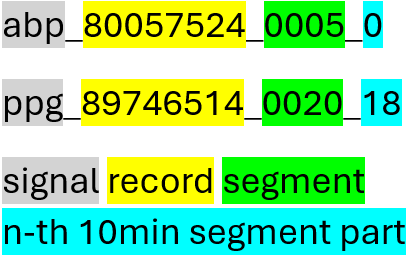
\includegraphics[width=0.3\textwidth]{images/methods/segments}
    \end{center}
    \vspace*{-7mm}
    \captionsetup{format=plain, justification=centering}
    \caption{\small Examples of extracted segment files}
    \label{fig:segments}
\end{wrapfigure}

As noted earlier, each subject in the database may encompass multiple studies, records, and segments.
To prevent disproportionate representation of individual patient data, a limit of 100 segments, each spanning 10 minutes, was imposed per subject.
This is specifically important for data retrieval from the MIMIC-III database, which is intended for training and testing purposes.
However, this restriction was not applied to data retrieval from the MIMIC-IV database, which is designated for validation purposes and aims to encompass all available 10-minute segments, thus simulating real-world data where over-representation is not a concern.

\begin{wrapfigure}{r}{0.35\textwidth}
    \vspace*{-5mm}
    \begin{center}
        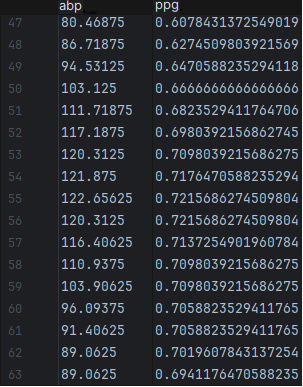
\includegraphics[width=0.3\textwidth]{images/methods/values}
    \end{center}
    \vspace*{-7mm}
    \captionsetup{format=plain, justification=centering}
    \caption{\small Example raw ABP and PPG values}
    \label{fig:values}
\end{wrapfigure}

Additionally, the primary objective was to achieve a dataset split ratio of 60/20/20 for training, testing, and validation, where 80\% of the data comprises the MIMIC-III dataset for training and testing (60/20), and the remaining 20\% consists of the MIMIC-IV dataset for validation purposes.
To facilitate this, an initial set of x segments was retrieved from the MIMIC-IV database, followed by obtaining four times the number of x segments from the MIMIC-III database.
However, it is important to acknowledge that the quantity of segments obtained from each database doesn't directly correspond to the number of features utilized in the ML phase, as signal processing (SP) tasks are performed in between.
Thus, the 60/20/20 split ratio for training, testing, and validation serves more as a guideline than an absolute target for the number of segments retrieved.
Details on achieving the actual proportions are provided in the subsequent section~\ref{subsec:sp_methods}.

\subsection{Signal Processing}
\label{subsec:sp_methods}

After the initial Data Preparation phase, the Signal Processing follows.
Its code is written in the \texttt{sp\_scripts.py} file.
The main \texttt{process\_data()} method is made up of these 6 steps (description and corresponding Python code):
\begin{enumerate}
    \item reading the fetched waveform data, \newline
    \small \texttt{seg\_name,raw\_abp,raw\_ppg = read\_seg\_data(filename,bp\_path,ppg\_path,fs)}
    \item \normalsize preprocessing the data, \newline
    \small \texttt{abp\_filt,ppg\_filt = pre\_process\_data(raw\_abp,raw\_ppg,fs,seg\_name)}
    \item \normalsize determining beats and heart rate (HR), \newline
    \small \texttt{abp,ppg,abp\_beats,ppg\_beats = signal\_processing(seg\_name,abp\_filt,ppg\_filt,fs)}
    \item \normalsize identifying fiducial points, \newline
    \small \texttt{abp\_fidp = fiducial\_points(abp,abp\_beats, fs) \newline ppg\_fidp = fiducial\_points(ppg, ppg\_beats, fs)}
    \item \normalsize extracting relevant features, \newline
    \small \texttt{features = extract\_features(abp\_fidp,ppg\_fidp,abp,ppg,fs,median\_window)}
    \item \normalsize saving extracted features. \newline
    \small \texttt{save\_split\_features(tot\_abp\_values,median\_abp\_values,tot\_ppg\_values,median\_ppg\_values)}
\end{enumerate}

The first and last steps simply involve the reading and writing of data utilizing the \textit{Pandas}~\cite{PandasPythonData} library, hence they will not be expounded upon further.
Steps 2, 3, 4 and 5 employ the \textit{NumPy}~\cite{NumPy}, \textit{Matplotlib}~\cite{MatplotlibVisualizationPython} and \textit{SciPy}~\cite{SciPy} libraries.
The following subsections delve into a comprehensive description of each subsequent step.

\subsubsection{Pre-Processing}
\label{subsubsec:filtering}

As previously delineated in the theoretical background section on Signal Processing(~\ref{subsubsec:signal_processing}), Data Pre-Processing or Filtering is a key component for ensuring a coherent projection of PPG and BP waveforms, as well as for their subsequent utilization.
A total of 8 filtering methodologies were experimented with to identify the optimal approach for this project:
\textit{Gaussian} and \textit{Gaussian Median}, \textit{Savitzky-Golay}, \textit{Butterworth} (\& lowpass),
\textit{Chebyshev II} (\& lowpass) and a manually created \textit{Whiskers} filter.
All filters and their parameters can be found in the appendix section~\ref{subsec:code_filters}.

In Figure~\ref{fig:filters}, effects of the named filtering techniques are displayed.

In order to identify the optimal filtering approach, several objective criteria had to be made.
For one, the amplitudes of the waveform should not be distorted, so that meaningful and rational values may still be extracted.
Secondly, the shape of both the ABP and the PPG waveform has to resemble a realistic pulse waveform (as for example shown in Figure~\ref{fig:acdc}), showing both the peak and the dip of the pulse wave.
Thirdly and ideally, the shape of a dicrotic notch should be visible in both the ABP and the PPG waveform.

% \newpage
\begin{figure}[h]
    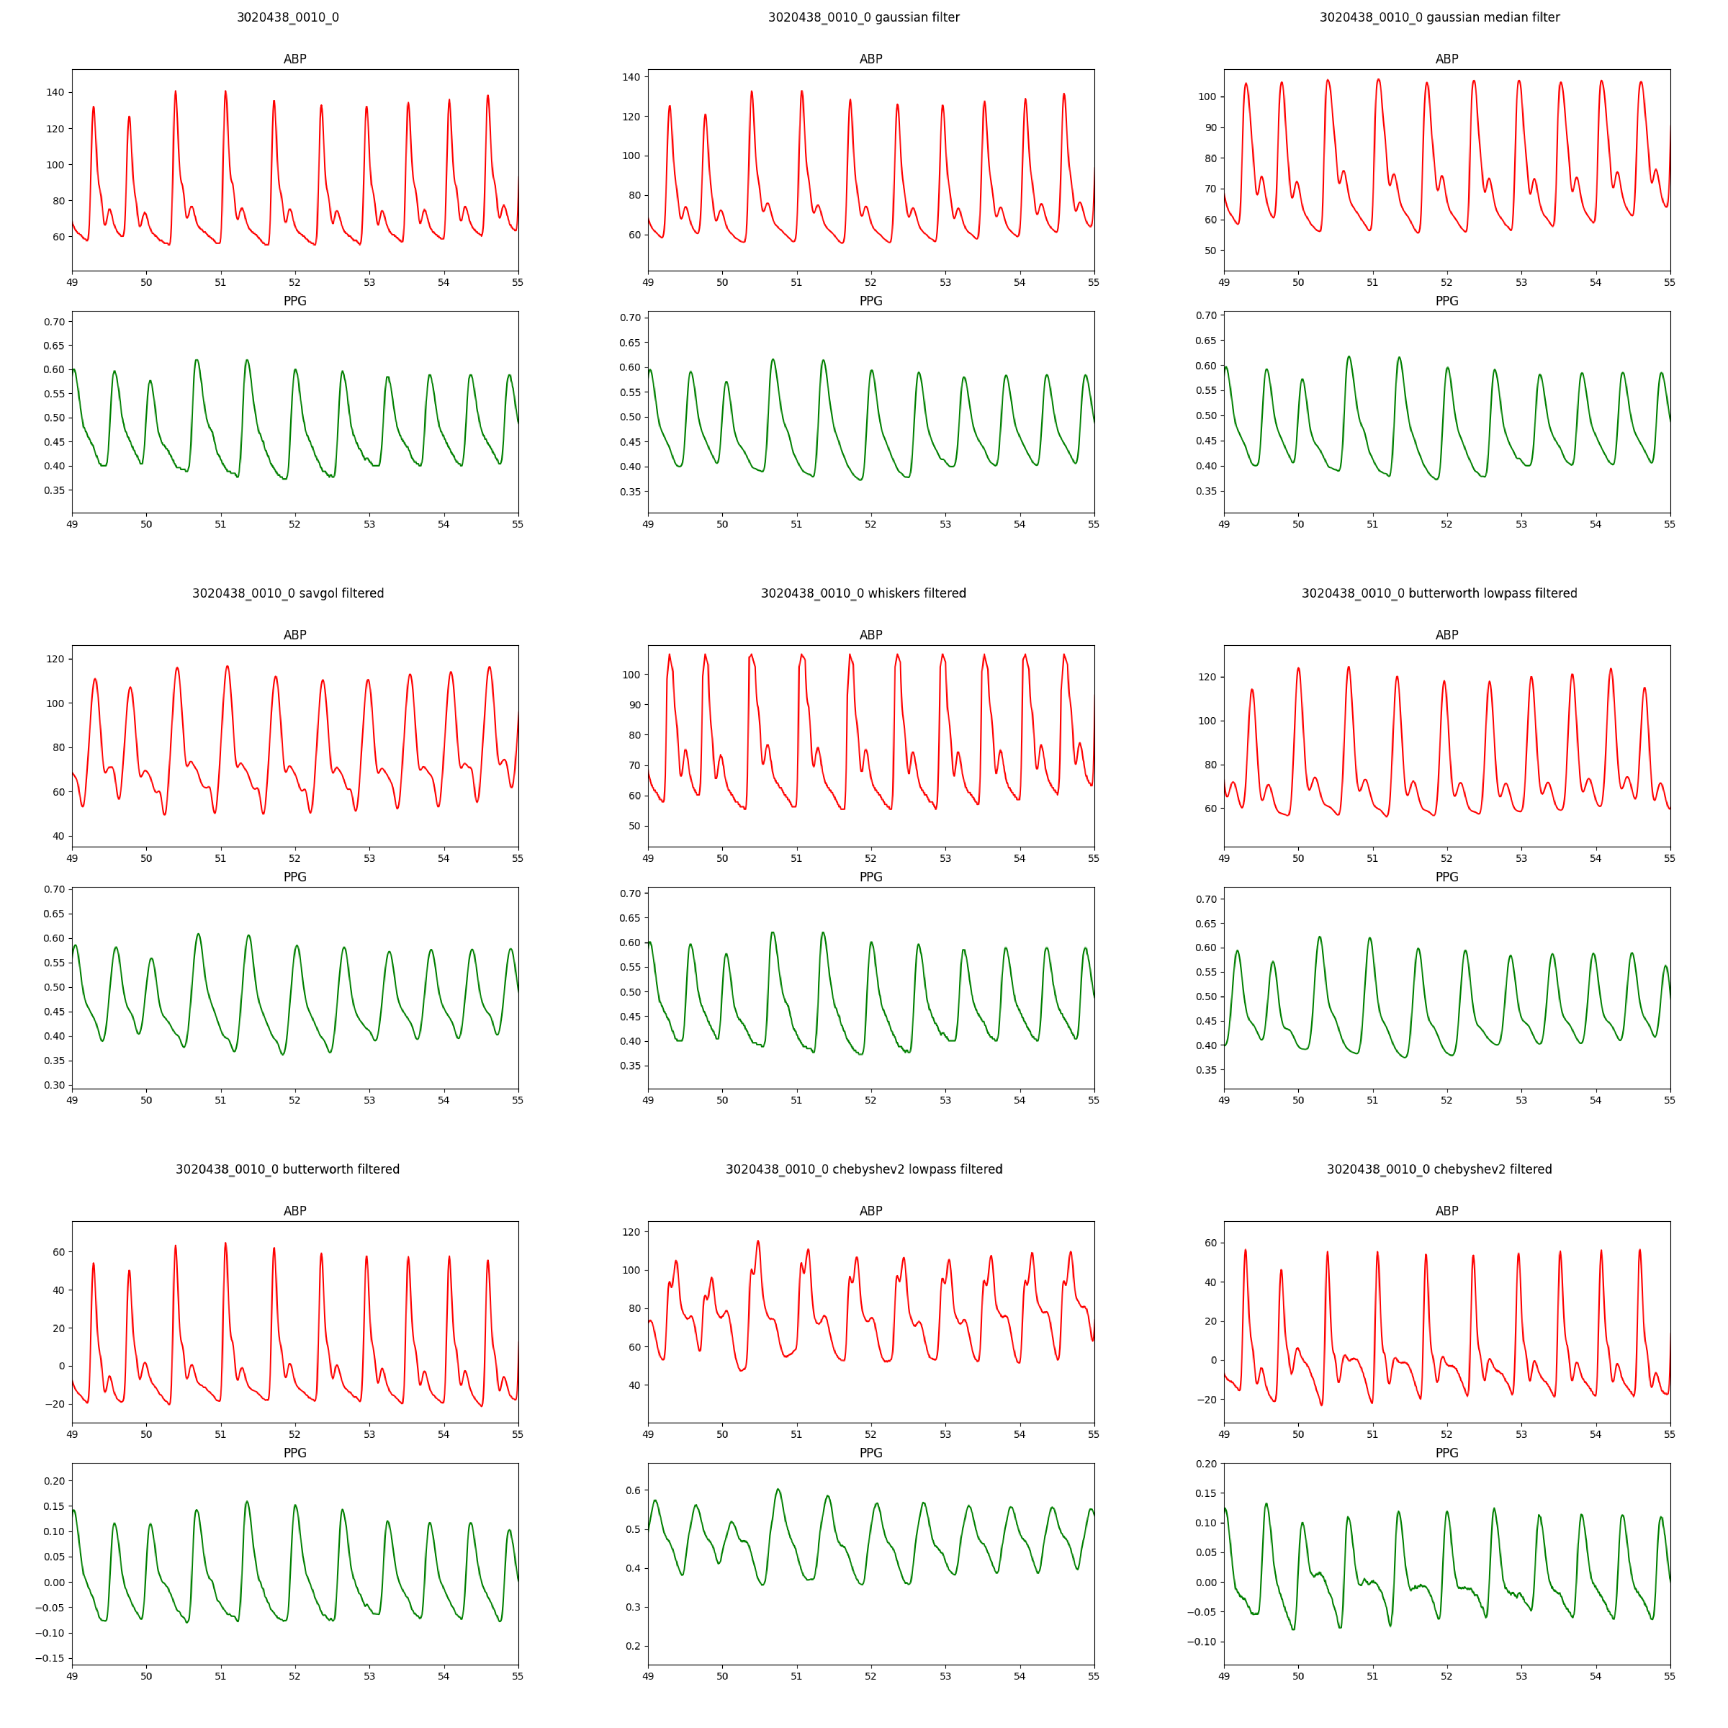
\includegraphics[width=0.9\textwidth]{images/methods/filters}
    \caption{9 different filters applied to the same ABP and PPG segment}
    \label{fig:filters}
\end{figure}

After a careful assessment of a larger sample of filtered waveforms the following approach was chosen as optimal:
%TODO add optimal filtering approach
butter + savgol optimal, because PPG shapes best (show pic)

\subsubsection{Beat Finding Algorithms}
\label{subsubsec:beats}

The third stage of the signal processing phase involves Beat Detection, which is crucial for precisely identifying waveform peaks, facilitating the accurate extraction of fiducial points.
Moreover, precise beat detection enables the segmentation of the waveform into individual pulse waves, extending from pulse onset to offset, which is essential for subsequent PWA procedures.

The beat detection reference code was obtained from the openly available MIMIC WFDB Tutorial~\cite{charltonMIMICWFDBTutorials2022}.
Elisa Mejía-Mejía from City, University of London authored the \texttt{pulse\_detect()} method, which is publicly accessible in the \enquote{Tutorials/Beat detection/Functions} directory.
This method offers four distinct algorithms: \textit{HeartPy}~\cite{vangentHeartPyNovelHeart2019}, \textit{Second derivative maxima}~\cite{elgendiSystolicPeakDetection2013},
\textit{Systolic upslopes}~\cite{arguellopradaNovelLowcomplexityPeak2018} and \textit{Delineator}~\cite{aboyAutomaticBeatDetection2005}.
Each one of them is explained in more detail in the following paragraphs.

\vspace{0.2cm}
\textit{Beat Detection Algorithms}
\vspace{0.2cm}

For reference to the textual descriptions, the entire code of the following methods can be found in the appendix~\ref{subsec:code_beats}.

The \textit{HeartPy} beat detection algorithm identifies peaks in a pulsatile signal by comparing each data point to a moving average,
then determines inter-beat intervals based on the detected peaks, with the option for peak correction based on segment length.
The algorithm exhibited poor performance with the provided MIMIC datasets, detecting peaks inconsistently and occasionally crashing during operation,
consequently rendering it unsuitable for further integration.

The \textit{second derivative maxima} (also called the \textit{d2max}) algorithm applies a bandpass filter to the input pulsatile signal,
squares the filtered signal, and then identifies blocks of interest (BOIs) based on thresholding.
Within each BOI, it searches for peaks and selects the highest peak as the position of the inter-beat interval.

The shortest method \textit{upslopes} detects inter-beat intervals by analyzing upslopes in the input pulsatile signal.
It sets a threshold for identifying peaks based on the rate of upslope changes.
Peaks are detected when the upslope exceeds a certain threshold, and the position of each peak is recorded as the starting point of an inter-beat interval.

The last default algorithm, known as \textit{delineator}, processes waveforms by filtering the signal, computing thresholds based on peak and trough amplitudes,
and detecting peaks and onsets using predefined criteria.
It refines the detected peaks and onsets to improve accuracy and outputs the positions of the starting points of inter-beat intervals.

Precisely these last 3 methods were all implemented for beat finding.
Throughout the developmental stage, it became evident that these distinct methods exhibit considerable variability in beat detection, thereby preventing the selection of a singular method as the optimal choice.
A comparison algorithm was then initiated to assess these algorithms for every single waveform.

The performance comparison involved an automated analysis of the average number of detected pulses generated by each method, followed by the calculation of the difference between ABP and PPG pulses, with preference given to the method yielding the smaller discrepancy.
However, beyond mere discrepancy size, the overall size of the beat arrays also factored into the selection process.
Any method producing beat arrays significantly larger or smaller than the other two was regarded as an outlier and deemed unsuitable for the specific waveform.
Ultimately, the optimal beat array was determined based on the \enquote{difference percentage} measure, which is computed as the percentage ratio of the absolute difference between ABP and PPG pulses to the total pulses from both signals.
Thus, the optimal method was identified as the one generating larger beat arrays and exhibiting smaller differences between PPG and ABP\@.

One new method, termed \enquote{mean crossings}, was devised manually by the author.
This method involves computing the mean value of a signal, identifying crossings above and below this mean,
tallying their occurrences to determine a beat interval, and employing it as a variable for minimum distance to detect peaks in the signal.
\enquote{Mean crossings} was considered optimal only when its resultant beat arrays were larger in size and exhibited smaller inter-signal differences.

Examples for the results of each algorithm applied to different waveforms are illustrated in Figure~\ref{fig:beat_algos}, with black dots representing the detected pulse beats.

\begin{figure}[h]
    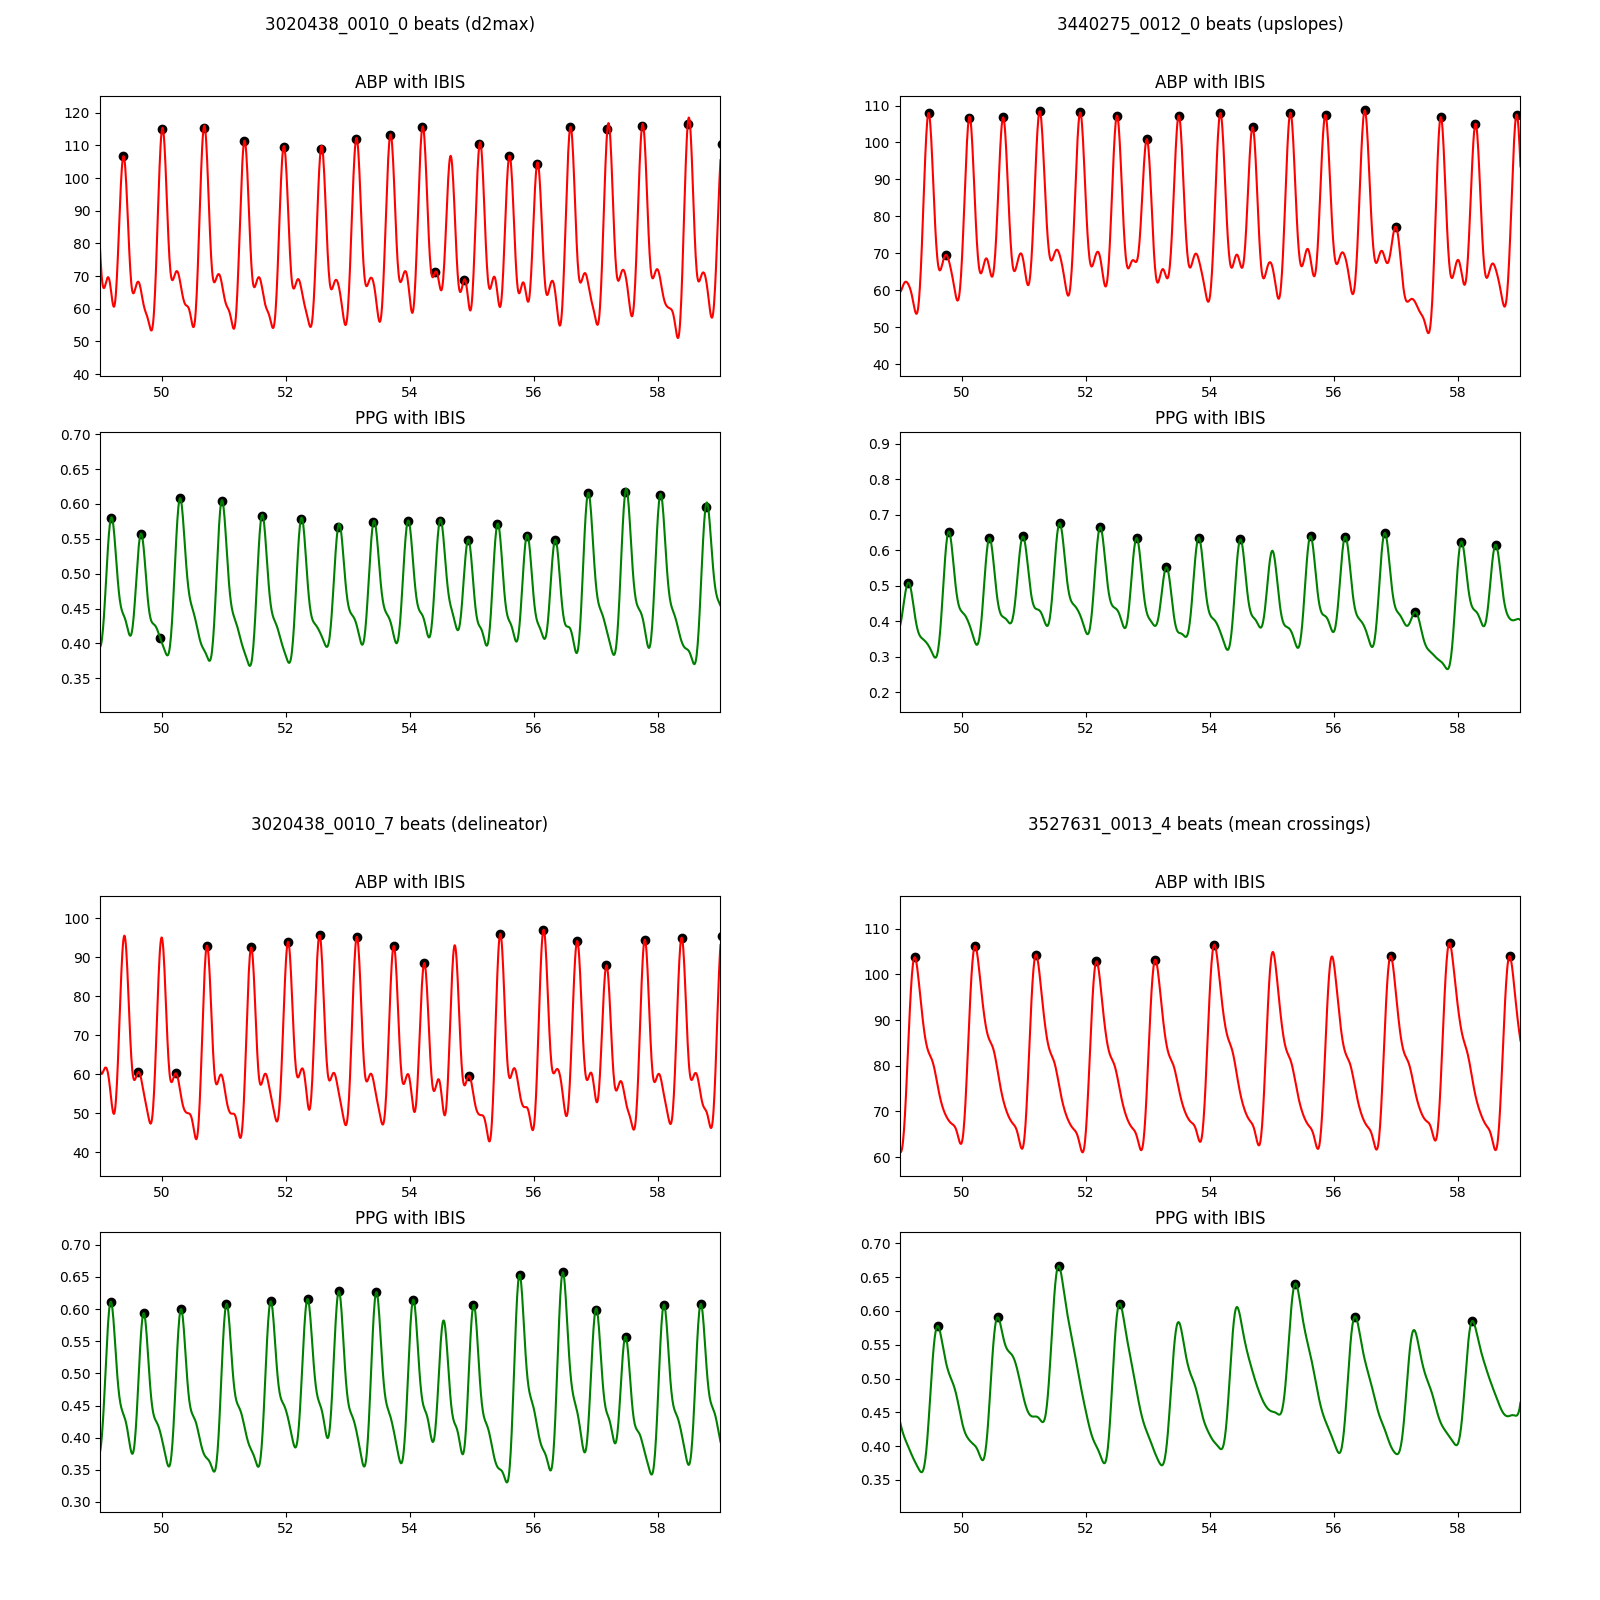
\includegraphics[width=0.9\textwidth]{images/methods/beat_algos}
    \caption{Application of 4 different beat finding algorithms}
    \label{fig:beat_algos}
\end{figure}

\vspace{0.2cm}
\textit{Selected Approach}
\vspace{0.2cm}

As already hinted in the description of the \enquote{mean crossings} algorithm, the optimal beat arrays were not utilized as the actual reference for beat timestamps, but solely for calculating the beat interval.
This was carried out to obtain a single variable, namely the \texttt{distance} parameter in a SciPy peak-finding function.
Experimentation revealed that this standard method was the most effective in identifying peaks in a waveform signal, and it was further refined using the \texttt{distance} and \texttt{prominence} parameters.
After trial and error, it was determined that three-quarters of the beat interval was the optimal \texttt{distance} value, while the \texttt{prominence} was set to 0.5 and 0.01 for ABP and PPG waveforms, respectively.
This methodology is illustrated in the following code snippet:

\vspace{0.1cm}
{\centering \texttt{abp\_beat\_interval = len(abp) / len(abp\_beats) \newline
ppg\_beat\_interval = len(ppg) / len(ppg\_beats) \newline
abp\_beats,\_=sp.find\_peaks(abp,distance=abp\_beat\_interval*.75,prominence=0.5) \newline
ppg\_beats,\_=sp.find\_peaks(ppg,distance=ppg\_beat\_interval*.75,prominence=0.01) \newline}}
\vspace{0.1cm}
\noindent and the improved accuracy of this approach is illustrated in Figure~\ref{fig:sp_beats}.

\begin{figure}[h]
    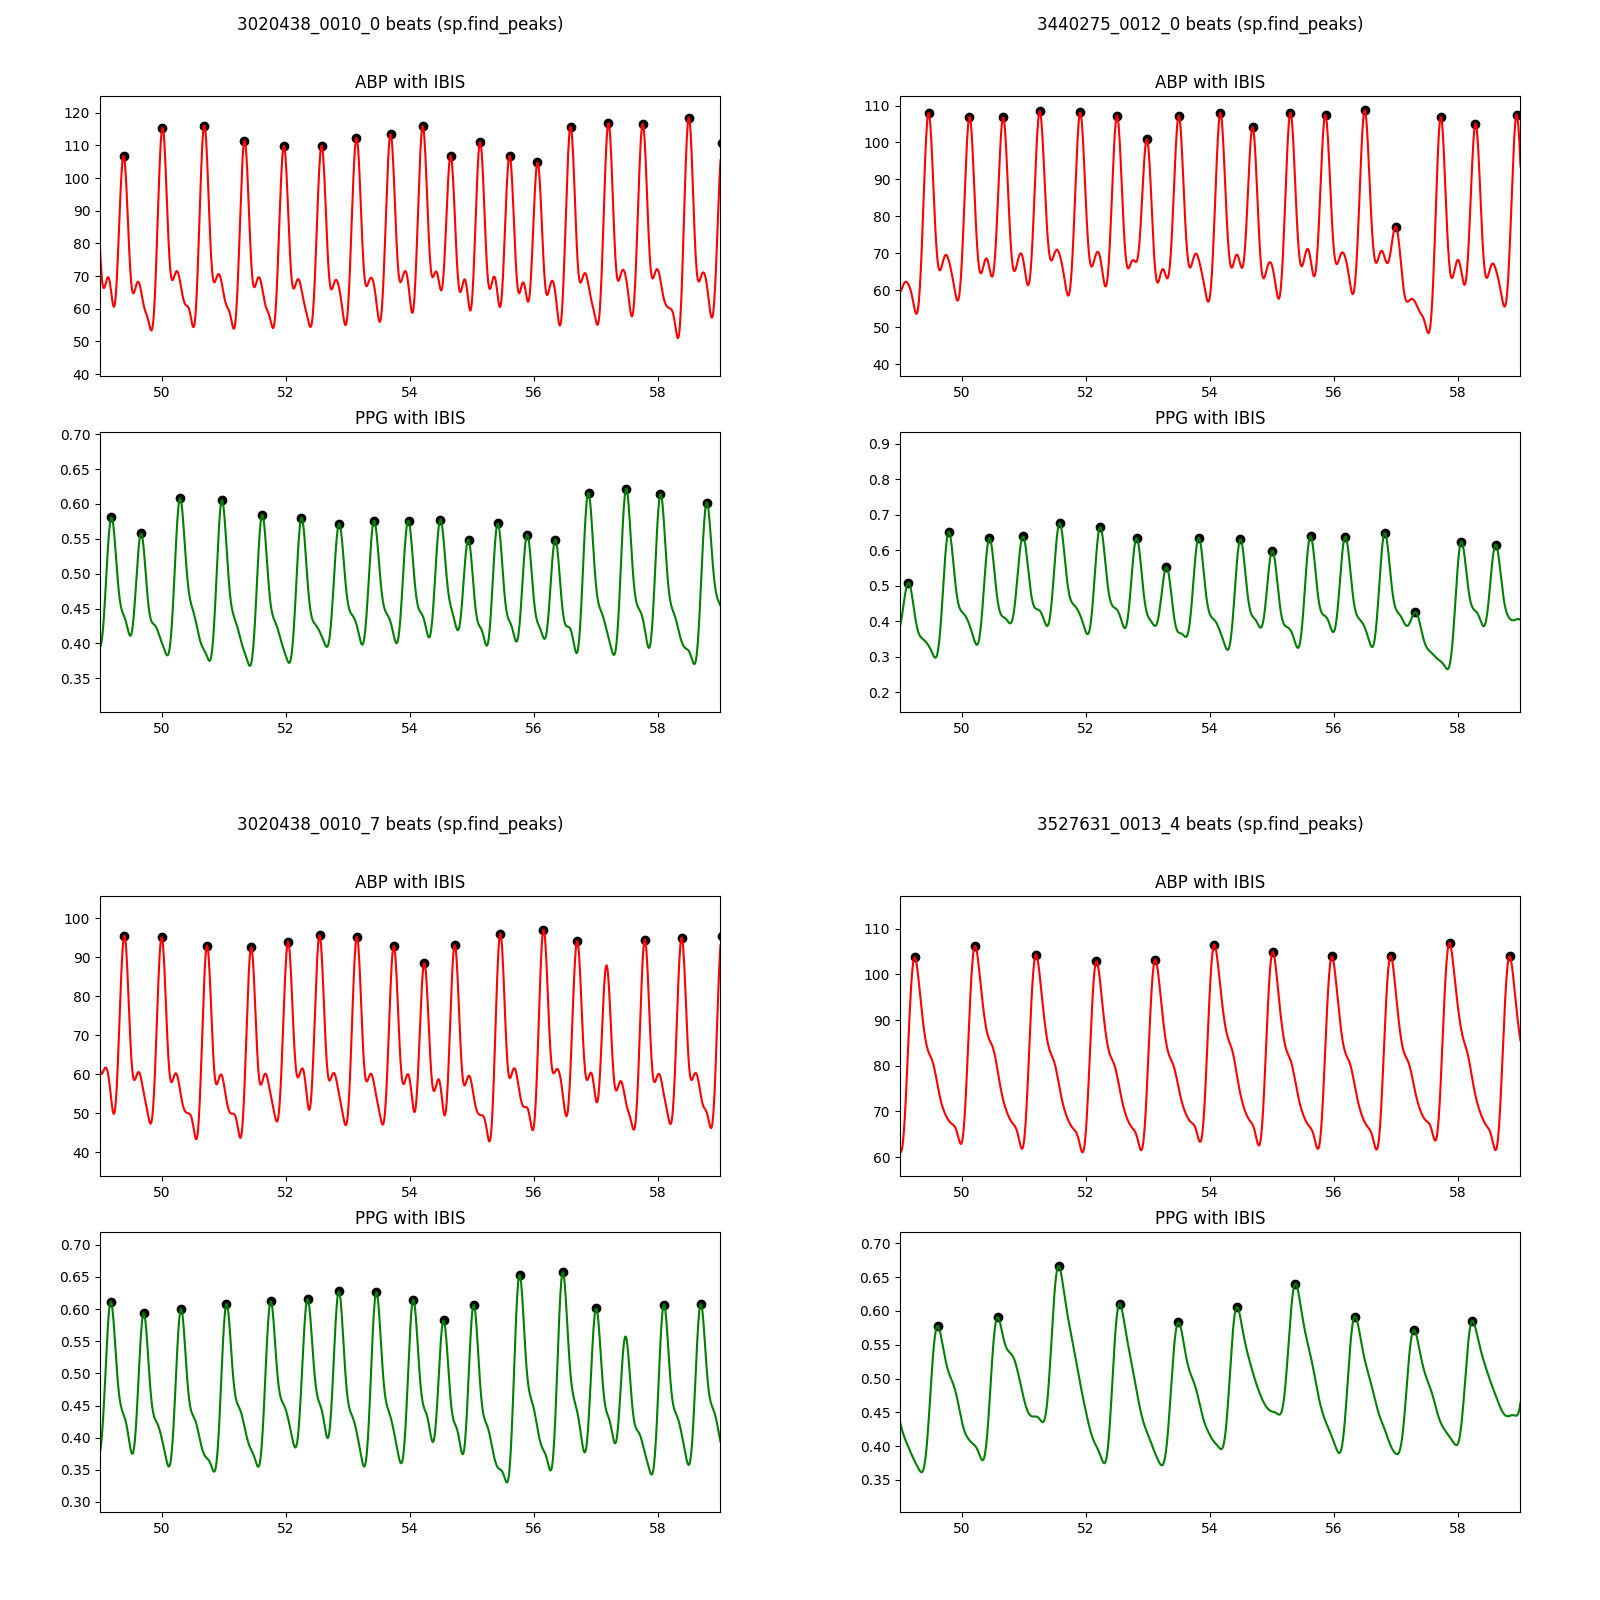
\includegraphics[width=0.9\textwidth]{images/methods/sp_beats}
    \caption{Application of the final beat finding approach on the same 4 waveforms as in Figure~\ref{fig:beat_algos}}
    \label{fig:sp_beats}
\end{figure}

In the rare event that this method also failed and fewer than 100 beats were found in the entire segment, the segment would be discarded, and the process would proceed to the next one.

\vspace{0.2cm}
\textit{Beat synchronization and grouping}
\vspace{0.2cm}

The final stage in generating an accurate beat timestamp array involves synchronization and grouping.

Due to a slight delay in the PPG waveform compared to the ABP signal (approximately 500 ms), synchronization becomes imperative.
This process entails identifying the closest PPG beat to the first ABP beat and vice versa, and the closest ABP beat to the last PPG beat.
Thereby splicing the respective arrays to produce two synchronized waveforms based on the indexes of the first and last PPG and ABP beats.

Additionally, it's crucial to address any instances of mis-detected beats in either signal.
For instance, if three ABP beats are detected at timestamps 50, 60, and 70, but only two beats are identified at timestamps 50 and 70 in the PPG waveform,
the ABP beat at timestamp 60 must be discarded as it lacks a corresponding PPG counterpart.
Consequently, the resulting beat arrays for both PPG and ABP waveforms possess identical lengths, with timestamps differing only marginally.

The effect of this final process is illustrated in Figure~\ref{fig:synchronized}.

\begin{figure}[h]
    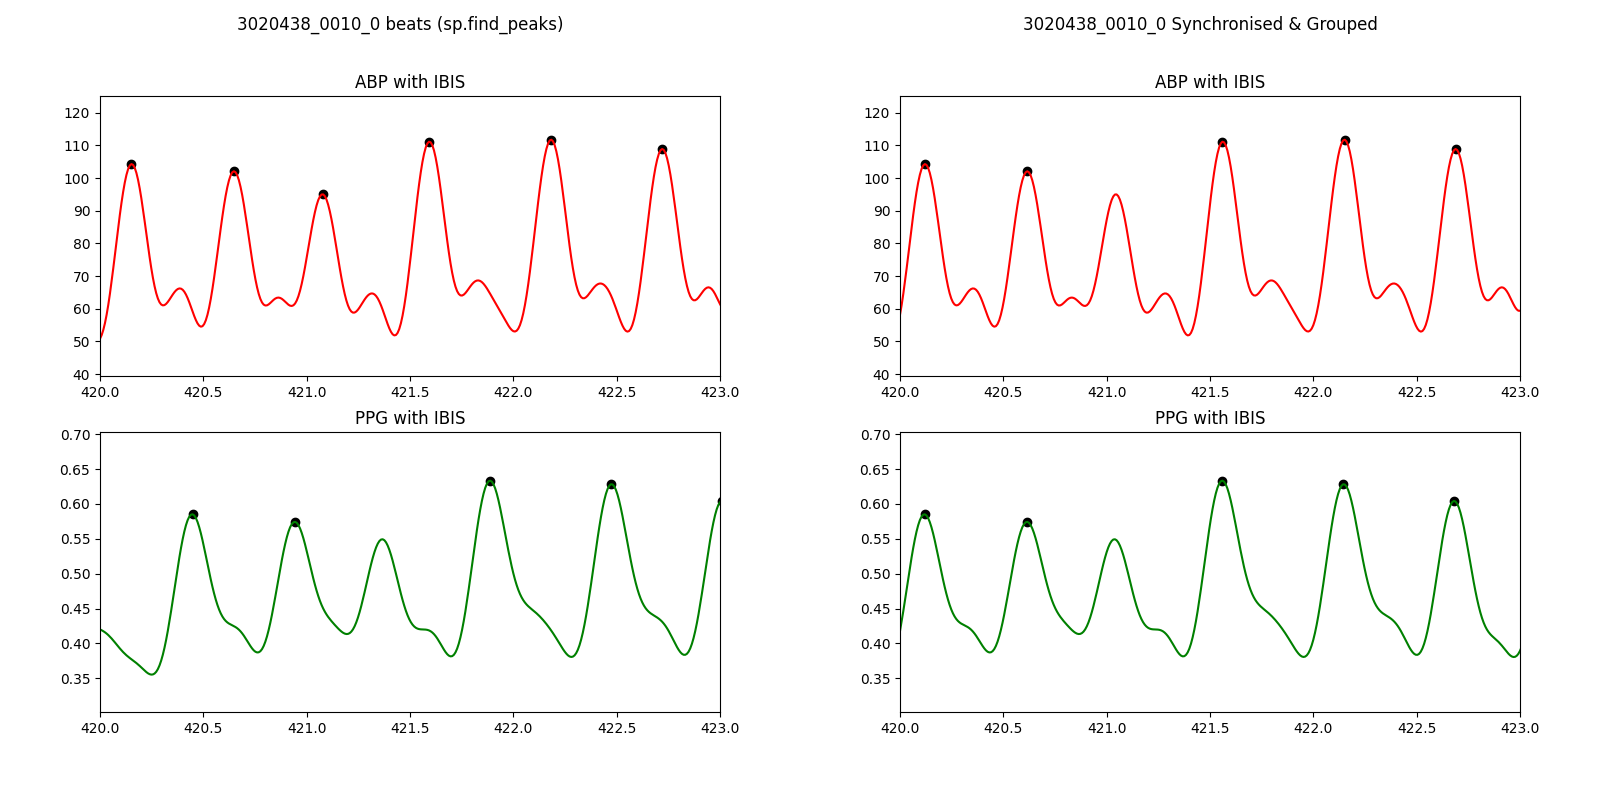
\includegraphics[width=0.9\textwidth]{images/methods/synchronised}
    \caption{Effect of beat synchronization and grouping}
    \label{fig:synchronized}
\end{figure}

\vspace{0.2cm}
\textit{Dealing with distorted signals}
\vspace{0.2cm}

An important aspect to highlight from the signal processing phase of the project is the management of irregular signals.
Two instances are depicted graphically in Figure~\ref{fig:distorted}.
The first plot exhibits a noticeable distortion in the PPG measurement, while the second plot likely portrays the waveform of a patient experiencing some form of arrhythmia.

\begin{figure}[h]
    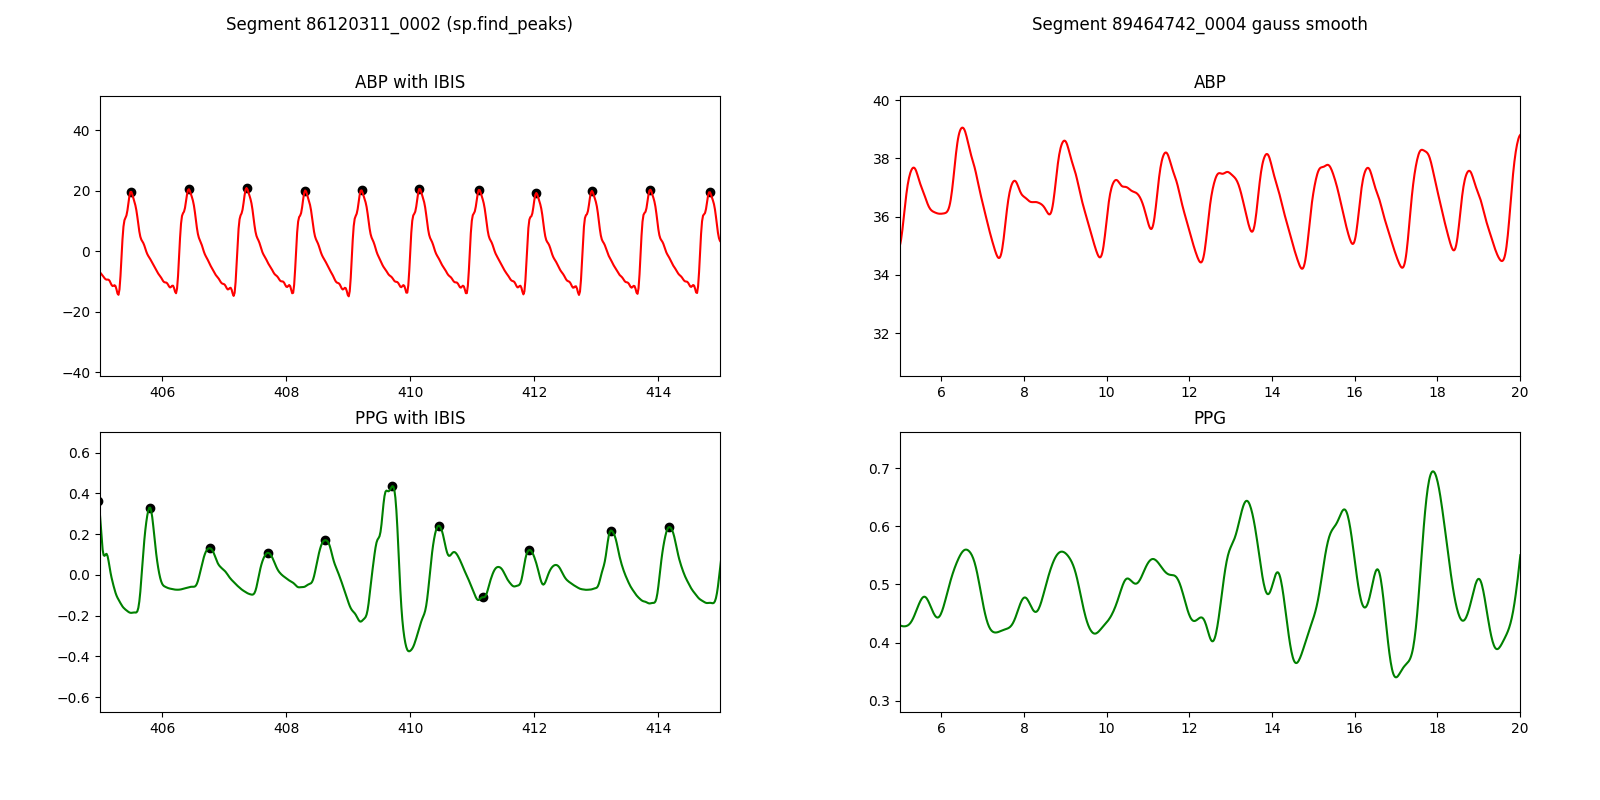
\includegraphics[width=0.9\textwidth]{images/methods/cringe_signals}
    \caption{Examples of distorted or irregular signals}
    \label{fig:distorted}
\end{figure}

In the scope of this project, manual selection of waveform shapes was not conducted, mainly due to the extensive size of samples.
Instead, the exclusion of irregular segments relied solely on programmed Exception Handling.
As previously discussed in the beat finding section, the rare occurrence of not finding 100 beats in a waveform may indicate a pathological heart function, as ensured by the following code:

\vspace{0.1cm}
{\texttt{\small if len(abp\_beats) < 100 or len(ppg\_beats) < 100: \newline
\indent\indent\indent raise Exception('Signal Processing failed: \newline
\indent\indent\indent\indent\indent\indent a substantial amount of beats not found')}}
\vspace{0.1cm}

Another issue occasionally encountered was the inconsistency in beat grouping.
This occurred when the beat finding algorithms generated arrays with significantly different beat timestamps, even post-synchronization.
If the beat grouping algorithm eliminated more than 5\% of the initial beats, it was considered a flawed array, leading to the exclusion of the current segment entirely.
This is exemplified by the following exception raised:

\vspace{0.1cm}
{\texttt{\small if (pre\_sync\_length) > (post\_sync\_length) * 1.05: \newline
\indent\indent\indent raise Exception('Signal Processing failed: \newline
\indent\indent\indent\indent\indent\indent too big of a difference after grouping')}}
\vspace{0.1cm}

\subsubsection{Fiducial Point detection}
\label{subsubsec:fidp}

The fourth phase within the signal processing phase encompasses the detection of Fiducial Points (FIDPs), which is directly linked to feature extraction.

As detailed in the background section~\ref{subsec:computing_background}, this approach focuses on identifying distinct landmarks within a single pulse waveform.
Similarly to Pulse Detection, the framework for this segment was derived from the MIMIC WFDB Tutorial~\cite{charltonMIMICWFDBTutorials2022}, which is publicly accessible in the \enquote{Tutorials/Pulse Wave Analysis/Fiducial Point Functions} directory.
The \texttt{fiducial\_points()} function is designed to identify and adjust pulse-related signals by recognizing various FIDPs within cardiac cycles,
including systolic peaks, onsets, diastolic peaks, maximum slopes, and specific points derived from the second and third derivatives of the pulsatile signals.
Leveraging signal processing methodologies from NumPy, SciPy, and Matplotlib libraries, it determines the positions of these FIDPs based on the input pulsatile signal, peak positions, and sampling rate.
Moreover, it provides visualization capabilities to examine the detected points and their magnitudes, facilitating further analysis and enhancement of the FIDPs list.
The visualization of this function is provided in Figure~\ref{fig:wfdb_fidp}.

\begin{figure}[h]
    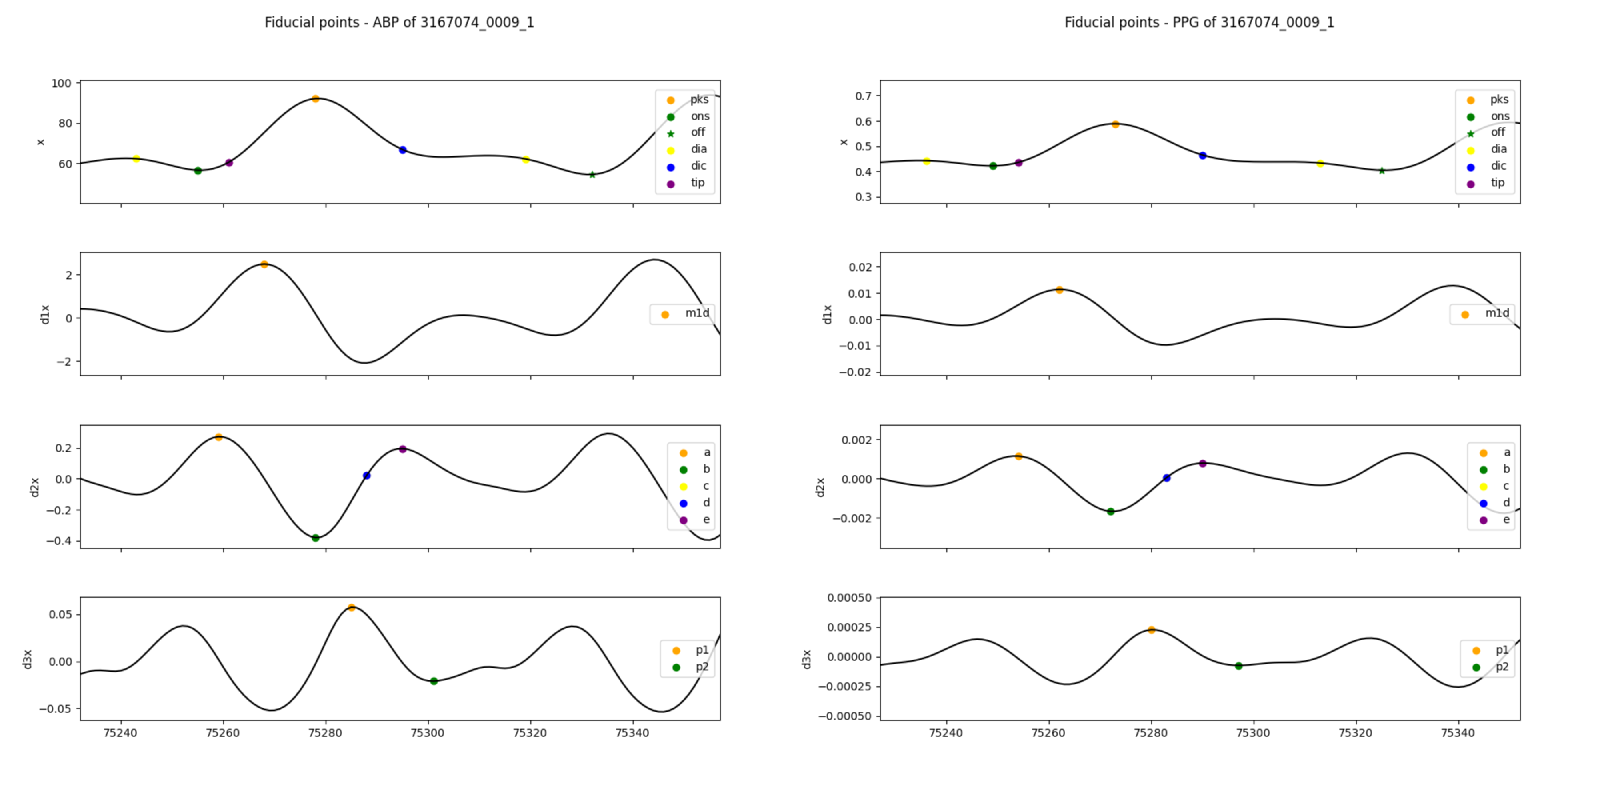
\includegraphics[width=0.9\textwidth]{images/methods/fidps}
    \caption{Example FIDP detection}
    \label{fig:wfdb_fidp}
\end{figure}

This method, akin to the pulse detection function, required refinement and enhancement to ensure smoother execution.
The details of these adjustments, along with the complete code, are available in the appendix~\ref{subsec:code_fidp}.

An important caveat to note pertains to the detection of the dicrotic notch.
As likewise discussed in the theoretical background section, the detectability of this fiducial point is greatly influenced by a patient's age and physical condition,
diminishing in clarity with advancing age and declining health.
Consequently, the extraction of fiducial points was constrained; not every waveform contained all the specified fiducial points (e.g., the dicrotic notch may have been absent).
Further insights into potential enhancements are provided in the discussion section~\ref{sec:discussion}.

\subsubsection{Feature Extraction}
\label{subsubsec:features}

The fifth and result-providing step of the signal processing phase is Feature Extraction.
It, as the name already hints at, is the most important part that provides the data for the creation and validation of ML models.
The methods of this section were created manually by selecting features on the basis of medical knowledge and past researches of this type~\cite{el-hajjDeepLearningModels2021, charltonAssessingHemodynamicsPhotoplethysmogram2022, maqsoodSurveyShallowDeep2022}.

\vspace{0.2cm}
\textit{PPG Features}
\vspace{0.2cm}

The following is a list of all extracted features from a single PPG pulse wave:
\begin{itemize}
    \item \texttt{sys}: the systolic peak amplitude value,
    \item \texttt{dia}: the diastolic dip, or lowest amplitude value after the systolic peak,
    \item \texttt{sys\_t}: systolic time - time difference between the systolic peak and the onset,
    \item \texttt{sys\_area}: systolic area - integral value of the signal over the time interval bounded by the onset and systolic peak,
    \item \texttt{dia\_t}: diastolic time - time difference between the offset and the systolic peak,
    \item \texttt{dia\_area}: diastolic area - integral value of the signal over the time interval bounded by the systolic peak and offset,
    \item \texttt{delta\_t}: delta time - time difference between the diastolic peak and the systolic peak,
    \item \texttt{delta\_area}: integral value of the signal over the time interval bounded by the systolic peak and the diastolic peak,
    \item \texttt{pulse\_area}: integral value of the signal over the time interval bounded by the onset and offset,
    \item \texttt{dia\_sys\_area\_ratio}: the ratio of diastolic area to the systolic area,
    \item \texttt{res\_index}: resistive index - ratio of difference between diastolic peak and offset values to difference between systolic peak and offset values,
    \item \texttt{vvi\_sys}: vessel volume fill-up (systolic) index - ratio of the systolic peak value to the maximum value among all systolic peaks,
    \item \texttt{vvi\_dia}: vessel volume drained (diastolic) index - ratio of the minimum value among all offset values to the offset value,
    \item \texttt{dw10}: diastolic width at 10\% amplitude - time duration between systolic peak and offset at 10\% pulse amplitude,
    \item \texttt{dw+sw10}: sum of diastolic and systolic widths at 10\% amplitude (systolic width is time duration between onset at 10\% amplitude and systolic peak),
    \item \texttt{dw/sw10}: ratio of diastolic width to systolic width both at 10\% amplitude,
    \begin{multicols}{6}
        \item \texttt{dw25} \columnbreak
        \item \texttt{dw+sw25} \columnbreak
        \item \texttt{dw/sw25} \columnbreak
        \item \texttt{dw33} \columnbreak
        \item \texttt{dw+sw33} \columnbreak
        \item \texttt{dw/sw33} \columnbreak
    \end{multicols}
    \begin{multicols}{6}
        \item \texttt{dw50} \columnbreak
        \item \texttt{dw+sw50} \columnbreak
        \item \texttt{dw/sw50} \columnbreak
        \item \texttt{dw75} \columnbreak
        \item \texttt{dw+sw75} \columnbreak
        \item \texttt{dw/sw75} \columnbreak
    \end{multicols}
    \item \texttt{mean\_frequency}: weighted average of positive frequencies in the magnitude spectrum obtained through the FFT,
    \item \texttt{total\_power}: sum of magnitudes of all frequency components in the FFT result, indicating the overall energy of the signal in the frequency domain,
    \item \texttt{normalized\_power\_at\_peak}: relative contribution of the peak frequency component to the total power of the signal computed through the FFT\@.
\end{itemize}

All features apart from the last 3 are extracted from the direct PPG pulse wave by calculating the values either from timestamps of the PPG amplitude values - all of them are regarded as time domain features.
The last three features are regarded as frequency domain features, since the values are calculated from the FFT, which is represented in the following function:

\begin{center}
    \begin{math}
        X(k) = \sum_{n=0}^{N-1} x(n) e^{-i 2\pi kn/N}
    \end{math}
\end{center}

\begin{flushleft}
    \small
    \begin{tabular}{ll}
        $X(k)$      & : Discrete Fourier Transform (DFT) coefficients at frequency index $k$ \\
        $x(n)$      & : Input signal data point at time index $n$                            \\
        $N$         & : Total number of samples in the input signal                            \\
        $k$         & : Frequency index ranging from $0$ to $N-1$                               \\
    \end{tabular}
\end{flushleft}

The code for the extraction of each feature can be found in the appendix~\ref{subsec:code_fe}.
The visualization of time and frequency domain features can be found in Figure~\ref{fig:td_feats} and~\ref{fig:fd_feats} respectively.

\begin{figure}[h]
    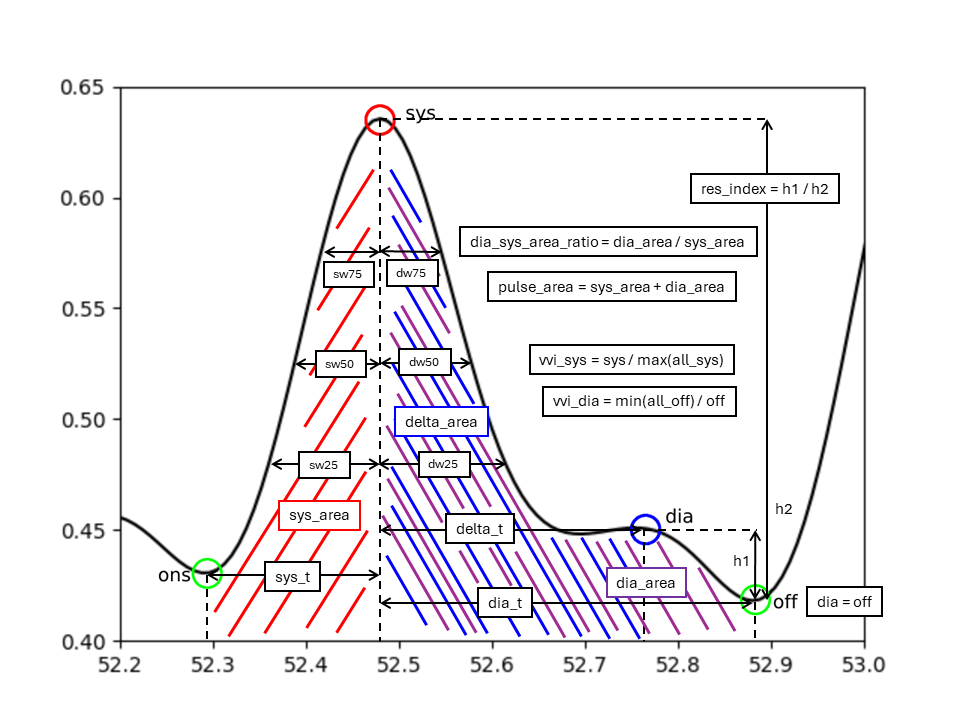
\includegraphics[width=0.9\textwidth]{images/methods/feats}
    \caption{Time domain features}
    \label{fig:td_feats}
\end{figure}

\begin{figure}[h]
    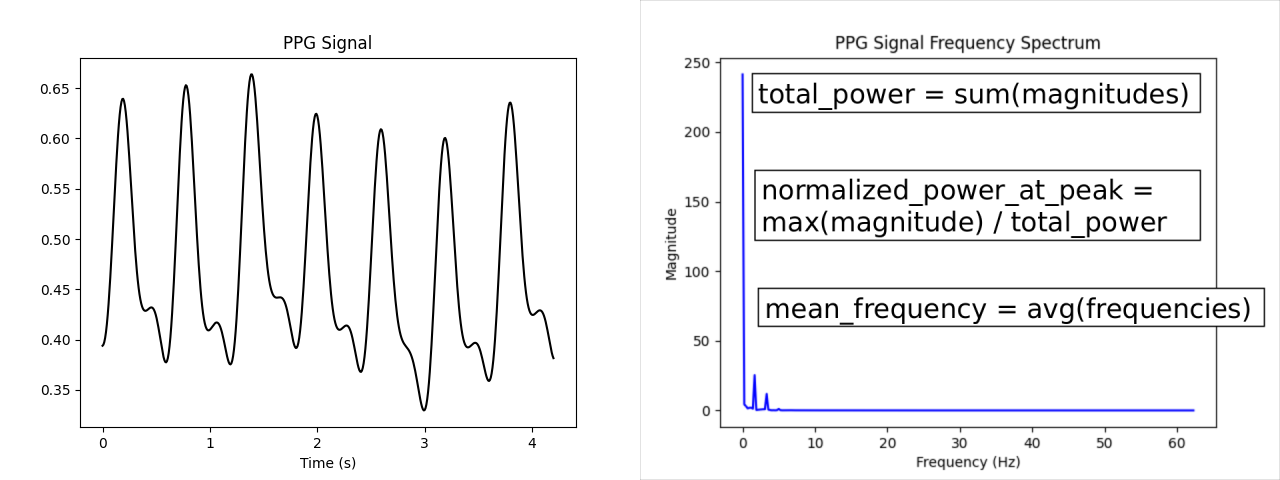
\includegraphics[width=0.9\textwidth]{images/methods/median_fft}
    \caption{Frequency domain features}
    \label{fig:fd_feats}
\end{figure}

\vspace{0.2cm}
\textit{ABP Features}
\vspace{0.2cm}

Three specific features were selected for extraction from the ABP waveform to serve as the target prediction values.
These features encompassed the Systolic Pressure (SP), Diastolic Pressure (DP), and Mean Arterial Pressure (MAP).
The determination of the SP and DP involved a straightforward method of extracting the values of the \texttt{sys} and \texttt{off} FIDPs (see Figure~\ref{fig:wfdb_fidp}).
Lastly, the calculation method employed for the MAP values was based on the formula provided by DeMers and Wachs~\cite{demersPhysiologyMeanArterial2024}:

\vspace{0.1cm}
{\centering  \large \texttt{MAP} = \texttt{DP} + \left(\frac{\texttt{SP} - \texttt{DP}}{3}).\right \par}
\vspace{0.1cm}
\normalsize

\vspace{0.2cm}
\textit{Total and median values}
\vspace{0.2cm}

The last step taken in the feature extraction, was the median value extraction over a specific beat window.
Measuring the median values over a specific PPG window offers several advantages over simply taking the absolute values from every single pulse wave.
Firstly, calculating the median helps to mitigate the influence of outliers or irregularities in individual pulse waves, providing a more robust representation of the underlying physiological state.
By capturing the central tendency of the data within each window, the median value offers a more stable and reliable estimate of the overall signal characteristics.
Additionally, median values effectively filter out any left-over noise from the pre-processing part, making them more reliable measures compared to absolute values.
Finally, this approach reduces the computational complexity compared to dealing with total features extracted from each pulse wave individually, making it more efficient for large-scale data processing tasks, such as ML model training.
Specifically these median values were the ones used in all subsequent ML processes.

Through empirical investigation, it was determined that a window of 7 consecutive beats served as the most effective median interval
for computing feature values from both PPG and ABP signals.
Within this interval, the median values for all features were computed, with the exception of frequency domain features.
For the frequency domain features, the FFT was applied to the entire 7-beat window, extracting values from the complete segment as illustrated in Figure~\ref{fig:fd_feats}.

\subsection{Machine Learning}
\label{subsec:ml_methods}

In this concluding section detailing methods, the utilization of Machine Learning methodologies is elaborated upon,
drawing from a range of studies as referenced in the background section~\ref{subsubsec:machine_learning}.
This study employed diverse models, distinct strategies for data splitting, and methods for training and validation.

The use of \textit{Scikit-Learn}~\cite{ScikitlearnMachineLearning} (version 1.4) was employed for simpler regression models within this study.
Utilizing version 2.2 of \textit{PyTorch}~\cite{PyTorch}, the library was enhanced with the CUDA toolkit for GPU acceleration in the context of NN processes.
The library \textit{wandb}~\cite{Wandb} was employed for the purpose of monitoring and visualizing the model's performance.

Initially, the PPG and ABP data were delineated as \texttt{X} and \texttt{y} correspondingly.
Then, data from the MIMIC-III DB was partitioned randomly adhering to the 80/20 training/testing proportions.
Following this, all data underwent normalization utilizing the \texttt{sklearn.preprocessing.StandardScaler} class.
This step was implemented to accommodate variations in feature scales and to guarantee an equal contribution of each feature to the analysis.

After this initial phase, the training of the models commenced.
A total of 8 regression models were implemented:
\begin{itemize}
    \item Linear Regression (\textit{PyTorch}),
    \item Multi-Layer Perceptron (\textit{PyTorch}),
    \item Long Short-term memory model (\textit{PyTorch}),
    \item bi-directional LSTM (\textit{PyTorch}),
    \item Gated Recurrent Unit (\textit{PyTorch}),
    \item bi-directional GRU (\textit{PyTorch}),
    \item Random Forest Regressor (\textit{Scikit-Lear})
    \item Support Vector Regressor (\textit{Scikit-Learn})
\end{itemize}

The code of the listed ML models can be found in appendix~\ref{subsec:code_ml}.


The ML models' code can be located in appendix~\ref{subsec:code_ml}.

In LR and MLP models, the utilized optimizers were \enquote{Stochastic Gradient Descent} (SGD)\cite{SGDPyTorchDocumentation} and \enquote{Adaptive Moment Estimation} (Adam)\cite{AdamPyTorchDocumentation} respectively.
The optimizer for LSTM and GRU models was \enquote{Limited-memory Broyden–Fletcher–Goldfarb–Shanno} (LBFGS) algorithm~\cite{LBFGSPyTorchDocumentation}, each running for 100 epochs with a learning rate set to 0.1.

The SVR model was initialized with the \texttt{linear} kernel, a regularization parameter \texttt{C} set to 100, and with an \texttt{epsilon} of 0.1.
The \enquote{RandomForestRegressor} model was configured with 100 decision trees, each restricted to a maximum depth of 10 nodes, and a minimum of 2 samples required to split an internal node.

During the training phase, the \enquote{Mean-Squared-Error} (MSE) loss was computed and used as the performance reference.
MSE is generally favoured in continuous value regression endeavors, because it gives more weight to larger errors, especially outliers.
For \textit{PyTorch} models, an \enquote{early-stopping} strategy was implemented, halting training if the testing loss did not improve for 3 consecutive epochs.

After the training step, an evaluation of feature importance was conducted, employing a method that assesses each feature's significance by permuting their values and observing the resulting impact on model performance.
This was followed by a subsequent identical iteration of the model, differing only by the incorporation of added weights to the most crucial features.

For the testing evaluation in both iterations, the chosen metrics included \textit{Root Mean-Squared-Error} (RMSE), \textit{Mean Absolute Error} (MAE), \textit{$R^2$} measure, \textit{Bias}, and \textit{Limits-of-Agreement} (LoA).

Finally, the dataset from the MIMIC-IV DB was utilized for model validation.
The same data normalization techniques were applied as in the training stage.
Following the prediction of ABP, the resulting dataset was split into three, encompassing the predicted values of SP, DP, and MAP\@.
RMSE and MAE values were calculated for the entire prediction dataset, as well as for each of the three separate predicted value arrays.
Precisely these metrics effectively portrayed the ultimate accuracy of the model in predicting ABP (SP, DP and MAP).
